\chapter{Background and existing work}

\todo[inline]{Fill out specific details of the items introduced in the previous chapter}


\todo[inline]{Add more motivation for probabilistic embeddings. For example, preview problem with existing algorithms: When embeddings are inferred, there are multiple sources of uncertainty and local optima leading to different representations which are equally valid. Implication for alignment is that extra information such as variance, can be helpful for disambiguation. }

\todo[inline]{Make more references to multi modal learning having a synergistic effect - reference multi task training \cite{DeepMultimodalEmbedding} and \cite{OverviewMultiTaskLearning}}

\section{Concepts}

There is a wide body of philosophical literature on the exact definition of a concept, but in this document we will focus on the definition from \cite{stanfordconcepts} of concepts as mental representations or psychological entities, as it is also a main definition used in cognitive science \cite{Pinker2007}. In \cite{NatureOfHumanConcepts}, concepts are related to human characterisation of categories of objects, noting that such categories may overlap and have fuzzy boundaries. In \cite{GOLDSTONE2002295}, concepts are defined not only by features (apple maps to 'red or green or yellow in colour', 'round in shape') - the ``external grounding" description of meaning, but also by their relationships to each other ('apple' is more like 'pear' but less like 'durian'). The ``conceptual web" description states that a concept's meaning is defined by its place in the structure of all concepts in the system. 

In the field of computer science, there exist many frameworks of concepts defined in machine-interpretable ways. Some notable examples are Cyc \cite{Cyc} (an ontology of ``common-sense" rules and concepts), WordNet (a lexical database of English words, with the inherent assumption that words and concepts are interchangeable) \cite{WordNet}, and the Google Knowledge Graph \cite{KnowledgeGraphs}. These are all based on the idea that relationships between entities in the systems are important and contain valuable information. 

There is precedent for this way of thinking in the psychological and cognitive science literature. In \cite{SHEPARD19701} it is found that the relationships between concepts (internal mental representations) should reflect the relationships between the external (real world) representations; this was experimentally tested by querying subjects on the identification of US states by shape. This was further confirmed by \cite{SecondOrderIsomorphismFaces}. \cite{GOLDSTONE2002295} found an algorithm that was able to use the internal relationships between concepts in disparate systems to find correspondence between those two systems. 

\cite{CoocurrenceVisionLanguage2021} found that object representations in the human brain (which can be thought of as concepts - mental representations) reflect the co-occurrence statistics of vision and language. They posit that objects occur in context, with certain sets of objects occurring together more often than not, and that the human brain possesses mechanisms to support this type of contextual knowledge. Their research found that brain response could be predicted based on visual and language (text) stimuli. \todo{Add how co-occurrence comes into this}. Research by \cite{STANSBURY20131025} supported this by showing that the brain's response to scenes could be predicted based on clusters of co-occurring objects in that scene. 

The prevailing body of research evidence thus suggests that concepts may be considered to embody observed phenomena or events in the world, and that the relationships between concepts are important. 

\section{Multi-task learning}

\cite{OverviewMultiTaskLearning} gives several reasons for why multi-task learning allows models to generalise better. By training on multiple tasks, the model can learn a more general representation of the pattern that underlies all those tasks. If this general representation is closer to the true underlying representation of the generative pattern for the data underlying all tasks, learning it will allow the model to generalise to novel tasks better. This representation is also less likely to overfit as it might be if it was trained only on one task, because multi-task learning also has a regularising effect by adding an inductive bias. 


\section{Embeddings}

In machine learning, embeddings are real-valued, continuous, vector representations of features, which themselves may conform to concepts or features. Language embeddings are the most commonly known types of embeddings (that is, they are built from textual input data), but may originate from any data. Embeddings are intrinsically a dimensionality reduction technique for representing potentially very high dimensional data in a lower dimensional space. One of the first word embedding algorithms is \texttt{word2vec} \cite{word2vec}, in which a neural network is used to learn embeddings from a corpus. The algorithm projects similar words to similar locations in the target vector space, taking advantage of co-occurrence patterns (some words occur in the neighbourhood of other words). The resulting embeddings should reflect the semantic properties of words. The ``Continuous Bag Of Words" (CBOW) variant uses a window of context (disregarding order) to predict the current word, and the Skip-gram variant uses the current word to predict the context window, weighted by distance from the current word. In both cases, we see that the context of the current word is important, pointing again to a relationship between concepts being used as input into embedding creation. 

The GloVe \cite{pennington2014glove} algorithm is another commonly used word embedding algorithm based on co-occurrence statistics. Embeddings are learnt based on co-occurrence statistics over an entire corpus, with the co-occurrence of a pair of words being augmented by 1 every time those words occur within a set context window of each other in the corpus. These algorithm can be generalised to learn embeddings from any source of co-occurrence statistics; in \cite{CoocurrenceVisionLanguage2021}, a set of object embeddings called \texttt{object2vec} was built from co-occurrence statistics from the ADE20K data set \todo{find citation} of images labelled by human annotators, using the \texttt{word2vec} algorithm. 

\cite{MikolovMachineTranslation} found that word embedding spaces have similar structure over different languages, even when those languages are linguistically quite far apart, like English and Vietnamese. This provides more support for the ideas in the previous section; that the relationships between nodes in the concept systems are significant. 

Most algorithms to learn embeddings have significant stochasticity, as they are often learnt by minimising loss using stochastic gradient descent. As with any such problem the loss function landscape is complex, and there are many local minima, with the solution being highly sensitive to initial conditions. Therefore, runs with different random seeds will produce different embeddings; not just the individual embedding values will differ, but also the relationships between those embeddings. In a later part of this document we show examples of this. 

\todo[inline]{FastText}

\todo[inline]{BERT, ELMo, etc}

A method of creating embeddings that does not use co-occurrence data is described in \cite{LaplacianEigenmaps}; it is a geometrically motivated graph-based algorithm. A weighted graph is created with a node for each point (concept), and edges are added between nodes if they meet some definition of closeness (such as Euclidean distance, or being in the $k$-nearest neighbour set). The embeddings are the eigenvectors of the graph Laplacian. This algorithm is also context-based but in a different way; it preserves local neighbourhood information and is shown to result in sensible clustering as shown with word embeddings created using it. 

All of the above algorithms result in deterministic embeddings; deterministic in the sense that each concept is represented by one vector of numbers (the embeddings themselves may generated in a non-deterministic fashion, in that many of the algorithms are based on neural networks which have a stochastic component to their learning). We can generalise the idea to probabilistic embeddings, in which each embedding is represented by multiple vectors that represent parameters of a prior distribution. For example we may consider embeddings to be multivariate Gaussians with independent dimensions (diagonal covariance matrix), therefore allowing us to represent each embedding as two $n$-dimensional vectors, one each for the mean and variance of the distribution. By learning the variance as well, we derive further information about each concept that can be used to quantify the degree of uncertainty of that concept in the system. \cite{ProbabilisticEmbeddingsCrossModal} represent cross-modal embeddings as probability distributions in embedding space, and use the uncertainty represented by the learnt variance in automated decision making. Including the uncertainty in their information retrieval task improved performance, as well as increased the interpretability of the final embeddings. Looking ahead to the problem of finding correspondences between embeddings in multiple domains, we also see that if there are two dimensions to each embedding, this can provide additional information for disambiguation during the mapping process. 

\cite{DensityMatchingWordEmbeddings} and \cite{vilnis2015word} learn word embeddings by modeling each embedding as a probability density function. \cite{DensityMatchingWordEmbeddings} learn bilingual embeddings in an unsupervised way by matching the densities of the two monolingual embedding spaces. This allowed them to achieve state-of-the-art results on linguistically distant language pairs without the special initialisation or complicated optimisation required by many unsupervised methods. \cite{vilnis2015word} learn a mapping from words and words in context to a Gaussian distribution over a latent space. This mapping is such that the linguistic and semantic properties of the words are preserved by the relationships between the distributions. Words that appear in similar context should have similar embeddings. In particular, they wished the entailment relationships (if there is an entailment relationship between A and B, A must imply B) to be represented by inclusion between the variances of A's and B's respective Gaussian distributions. 

\section{Alignment and ways to achieve it}
    
\subsection{Some definitions of alignment}

\subsubsection{Alignment as mapping two spaces to a single latent space}
In its simplest form, alignment requires learning to map between two vector spaces. The notation from \cite{ManifoldLearningTheoryAndApplications} is used here to state the problem, as we find it particularly clear.

If there are two datasets $X$ and $Y$ whose instances all lie on the same underlying manifold $Z$, one version of the alignment problem requires finding functions $f$ and $g$ such that $f(x_i)$ is close, for some problem-specific definition of distance, to $g(y_j)$.

\begin{figure}[H]
    \centering
    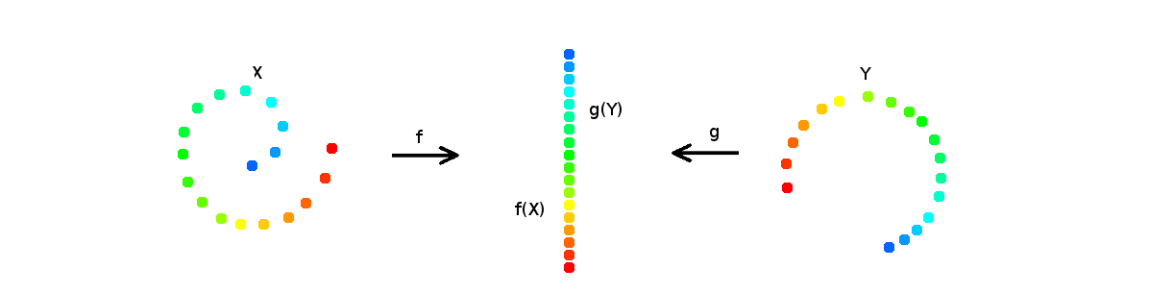
\includegraphics[width=0.9\textwidth]{images/review/alignment.png}
    \caption{
        Figure taken from \cite{ManifoldLearningTheoryAndApplications}. The $\vecX$ and $\vecY$ spirals denote the two datasets, with the center line showing the data points embedded into the shared space, with local similarity relations being preserved. $f$ and $g$ denote the functions mapping $\vecX$ and $\vecY$ respectively into the shared space. 
    }
    % generated by analyse.py 
\end{figure}

If $f(x_i) = g(y_j)$, then $x_i$ and $y_j$ are in correspondence. If we know ahead of time that $x_i$ and $y_j$ are analogous points in their datasets, then we can provide this information to the algorithm that is trying to infer $f$ and $g$. The union of the ranges of $f$ and $g$ is then the joint latent space. This can be generalised to more datasets than two. 

This however is a definition that maps both domains into the same space. 

\subsubsection{Alignment as learning mappings from one domain to another}

In the previous definition, alignment requires that both domains be mapped to a single latent domain. This can be useful for certain learning problems, for example to find a single language-independent representation of the data in multilingual related corpora. There is another definition for alignment, which requires only that domains can be mapped to each other without going through a single domain representation. 

\begin{figure}[H]
    \centering
    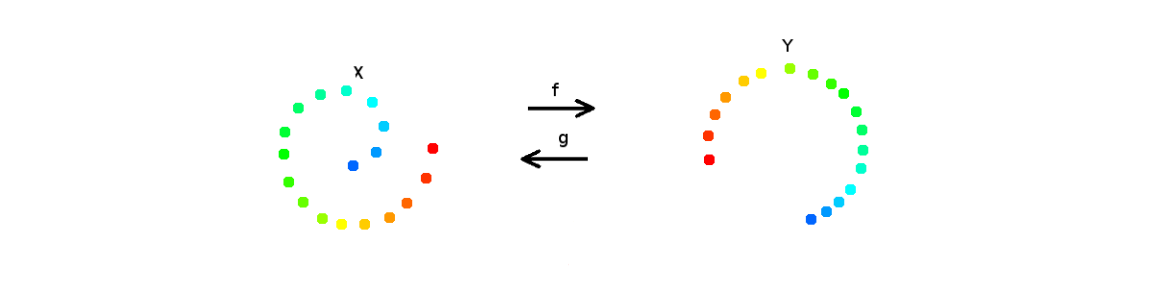
\includegraphics[width=0.9\textwidth]{images/review/alignment2.png}
    \caption{
        The $\vecX$ and $\vecY$ spirals still denote the two datasets, but this time $f$ and $g$ denote the functions mapping $\vecX$ and $\vecY$ respectively to each other, instead of into some shared space.
    }
    % generated by analyse.py 
\end{figure}

We wish to find mappings $f(\vecX) \rightarrow \vecY$ and $g(\vecY) \rightarrow \vecX$ where the spaces $\vecX$ and $\vecY$  have similar structures. This is slightly different from the definition of alignment in the previous section. 

\subsubsection{Second order isomorphism}

Returning to an idea first raised in \cite{SHEPARD19701}, we wish there to be second order isomorphism- functional relationships between clusters of concepts over the two modalities. Even if there is no structural resemblance between a concept and that concept's representation, the same structure should be observed between the relationships between the concepts  and the representations. As stated by \cite{GOLDSTONE2002295}, the meaning of a concept is highly tied in with its relationships to other concepts within that modality. Similarity relationships between concepts within the same system can therefore be used to translate, or map, between systems; using only these relationships, \cite{GOLDSTONE2002295} found an algorithm, ABSURDIST, that was able to translate between systems of concepts. Without constraints on the two systems, or even on the number of concepts present in each system, ABSURDIST was able to find translations using only similarity matrices that some some external agent (a German-English bilingual human, in the paper's example) had created. ABSURDIST found that while within-system relationships are enough to find a translation, this translation can be made more robust to noise by adding external, extrinsic information on correspondences (certain correspondences are weighted with higher values). 

\cite{GOLDSTONE2002295} found that ABSURDIST's mappings were better for systems that had a greater number of elements. This is because such a system has more similarity relations, and each similarity relation provides a constraint to uniquely identify each member. Therefore, systems with more elements are more constrained. \todo{Include ABSURDIST 2? https://www.aaai.org/Papers/FLAIRS/2004/Flairs04-110.pdf - graph matching}


\subsubsection{Applications of alignment problems}

Some examples of alignment problems are given below. They span a wide range of applications. 

\begin{itemize}
    \item Biological manifold alignment: \cite{magan} applies alignment using Generative Adversarial Networks \cite{GAN} to the problem of alignment of cell correspondence between cytometry batches.
    \item Bilingual lexical induction: \cite{wordtranslationwithoutparalleldata} applies alignment between word representations in single languages to derive a dictionary between those languages.
    \item Deep multimodal embedding: \cite{DeepMultimodalEmbedding} relates information from three modalities- point-cloud, natural language and manipulation trajectory data, to teach a robot arm  how to manipulate new objects. 
\end{itemize}

\subsection{Methods for concept alignment}

\subsubsection{Regression models}

Regression models are the simplest form of alignment model. They only require learning a transformation matrix $\vecW$ (possibly orthogonally constrained) from one domain to another, minimising mean squared loss $ \vecW f(\vecX) - \vecY$ which can then be applied to a new source vector to map into target space. \cite{MikolovMachineTranslation} uses this to find a ``translation matrix" that can map from word embeddings in one language space to another language space. Various standard preprocessing steps may be applied like normalisation to unit norm / mean centering, decorrelation to have unit variance, or SVD for dimension reduction.

\begin{itemize}
        \item Regression / orthogonal models: \cite{kalinowski2020survey} 
        \item Plus with various standard pre-processing steps:  
        \item Margin models: Still solving for alignment matrix W, reward weights associated with concepts that map directly but penalise the signal from other pairs. \cite{kalinowski2020survey} equation in Margin Models section. This is supposed to reduce ``hubness": Embeddings that have high similarity with everything in source or target space. This can be caused by some items being present in too many input data items (common frequency words, commonly present objects in pictures). 
        \item Loss functions that contain neighbourhood information: Relaxed Cross-Domain similarity local scaling, Locality preserving loss 
\end{itemize}

\subsubsection{Manifold alignment models}

As stated in \cite{ManifoldLearningTheoryAndApplications}, manifold alignment can be seen as a type of constrained joint dimensionality reduction with the aim of finding a low-dimension embedding of all the datasets, that preserves the topology of correspondences between them. Often, the datasets from multiple modalities will have disjoint features. The data may be of a very high dimension, but if data points all lie on a low-dimensional manifold, this manifold can be approximated by a graph and graph-theoretic methods can be used to align the lower-dimensional representations of all datasets. 

This of course requires the multiple datasets to be representable by a shared underlying structure. It may be convenient to simply learn the mapping from one dataset to another without ever formalising this shared structure, or it may be useful to find the common features. For example, in language translation it is often sufficient just to know the mappings from words or phrases in one language to the equivalent entities in another language. However if the problem is multilingual information retrieval, it may be more useful to express the translations of different documents in a single underlying joint representation. Our specific problem is learning aligned embeddings from co-occurrence data that represent the statistics of how concepts occur in different human-created media. If we consider the ultimate underlying generative process of all these media to be ``the real world", it is plausible to consider that the embeddings could have some underlying shared joint representation. 

Manifold alignment is obviously related to dimensionality reduction. Some existing techniques are Isomap \cite{Isomap}, which reduces dimension while preserving distances between points; locally linear embedding \cite {LocallyLinearEmbedding}, which reduces dimension while keeping distances the same between local neighbourhoods; and Laplacian eigenmap \cite{LaplacianEigenmaps}, which approximates the manifold by the adjacency graph derived from the embeddings \todo[inline]{fix this}. These algorithms all try to find the low dimensional embedding representation of a dataset. Manifold alignment simply uses these or similar algorithms to find embeddings for multiple datasets at the same time. If no correspondence information is given, manifold alignment will result in independent embeddings for each input dataset, but if direct correspondence information is provided, or a means for inferring such correspondence, manifold alignment will use that information to constrain the embeddings to be aligned. Manifold alignment considers each individual dataset to be part of one larger dataset whose range includes the mapped values of all other datasets. 

The specific technique for achieving this in \cite{ManifoldLearningTheoryAndApplications} starts by concatenating the graph Laplacians of all datasets as an approximation of the underlying manifold, then to use the Laplacian eigenmap algorithm mentioned earlier in \cite{LaplacianEigenmaps}. This algorithm requires finding the adjacency matrices of each dataset using a problem-specific similarity function, basically reducing the dataset to a graph. 

In \cite{UnsupervisedAlignmentWP}, an approach to aligning two sets of existing embeddings (learned separately from the alignment procedure) using a combination of Procrustes analysis and the Wasserstein distance is described. Procrustes analysis is normally used to learn a linear transformation between two sets of points with a known correspondence. If we consider $\vecX \in \R^{n \times d}$ ($n$ vectors of dimension $d$) and $\vecY \in \R^{n \times d}$ (another set of vectors of the same size), the Procrustes linear transformation is the solution to the following:

\begin{equation}
    \argmin \quad{\vecW \in \R^{d \times d}}  ||\vecX \vecW - \vecY||_2^2
\end{equation}

\cite{Goodall1991MI} used this to analyse two-dimensional shapes, where the shapes are considered to be the same if by application of rotation, translation and isotropic scaling, one can be transformed to the other. \cite{MikolovMachineTranslation} applied this technique to learn linear mappings between word embeddings in different languages using a bilingual dictionary. 

The Wasserstein distance, also known as the Earth Mover Distance, is the solution of the following optimisation problem

\begin{equation}
\begin{split}
    &\argmin{\vecP \in \mathscr{P}_n} \quad || \vecX - \vecP \vecY ||_2^2 \\
    \spaced{where}&\mathscr{P}_n = \{\vecP \in {0, 1}^{n \times n}. \vecP \one_n = \one_n, \vecP^T \one_n = \one_n \}
\end{split}
\end{equation}

If the source and target embeddings $\vecX$ and $\vecY$ are thought of as probability distributions, $\mathscr{P}_n$ denotes a permutation matrix that moves mass from $\vecX$ to create $\vecY$. 

\cite{Zhang2017EarthMD} used this distance measure as a minimisation objective to perform automated translation without supervision. By using the Wasserstein distance as a measure of distribution closeness, where the distributions are the source and target embedding spaces, they formulate a system in which minimisation of this distance draws the two distributions closer. The translation problem faced by \cite{Zhang2017EarthMD} did not have a one-to-one mapping between symbols, because some symbols in one space map to one symbol in the other space, therefore the minimisation of the objective had to be considered over the whole distribution. 

\cite{UnsupervisedAlignmentWP} combined both Procrustes analysis and the Wasserstein distance, to solve the following optimisation problem:

\begin{equation}
\begin{split}
\argmin{\vecQ \in \mathscr{O}_d} \quad \argmin{\vecP \in \mathscr{P}_n }\quad || \vecX \vecQ - \vecP \vecY||_2^2
\end{split}
\end{equation}

where $\vecQ$ is an orthogonal matrix. In order to practically solve this optimisation, they developed a novel stochastic algorithm to minimise a convex relaxation of this problem, details of which are omitted here. 

Point set or point cloud registration, is the manifold alignment problem applied to computer vision. As computer vision operates in 2 or 3 dimensions, many of its algorithms are specialised for that dimensionality and do not necessarily generalise well to alignment of embeddings with higher dimensionality. \todo[inline]{add more on this}

\subsubsection{Graph matching and graph similarity methods}

As described in \cite{kalinowski2020survey}, entities and relationships can be modeled as a graph. One example mentioned earlier in  \cite{ManifoldLearningTheoryAndApplications} defines adjacency matrices of each dataset using a problem-specific distance measure, where a weight is included in the matrix if one point is in the $k$-nearest neighbours of the other point. Once the relationships are represented as a graph, graph traversal algorithms can be used to learn about the structures. 

The general graph isomorphism problem, that of telling if two graphs represent the same structure, is NP-hard \cite{GraphIsomorphismNPHard}. There are polynomial-time algorithms for certain subtypes of graphs or trees \todo[inline]{take citations from \cite{kalinowski2020survey}}, but in general heuristic algorithms are the only practical possibilities. 

The \texttt{torch-two-sample} Python library and its corresponding paper \cite{torchtwosample} introduce smoothed versions of some graph-based similarity measures, the Friedman Rafsky test and k-nearest neighbours test, that can be used as loss functions for learning similar graph structures. These are not graph isomorphism methods per se, but rather aim to provide metrics for measuring how similar two distributions are based on graph-based properties.

\todo[inline]{Probably move this to appendix}

We introduce the following notation, which differs from that in \cite{torchtwosample} to avoid overloading previously defined terms in this document. 

\begin{itemize}
    \item $P$ is the distribution from which the points $X = \{\vecx_1, ..., \vecx_n \}$ are drawn.
    \item $Q$ is the distribution from which the points $Y = \{\vecy_1, ..., \vecy_n \}$ are drawn.
    \item $H(X) = (X, E)$ is the directed graph defined over the vertex set $X = \{\vecx_1, ..., \vecx_n \}$, with edges $E$.
    \item $J(Y) = (Y, F) $ is the directed graph defined over the vertex set $Y = \{\vecy_1, ..., \vecy_m \}$, with edges $F$. 
    \item These graphs are weighted with the distance function $d(\vecx, \vecx') = || \vecx - \vecx'||$, and we will denote with $d(e)$ the weight of the edge $e$ using distance function $d$. 
    \item For a labelling of vertices $\pi: X \rightarrow \{1, 2\}$ and any edge $e$ whose vertices $i$ and $j$ are adjacent, define $\Delta_{\pi}(e)$ to be 1 if $e$'s end points have different labels under the mapping $\pi$. 
\end{itemize}

The generic framework for the graph tests follows these steps:

\begin{enumerate}
    \item Let $Z$ be the union of the samples $X$ and $Y$ and let $K(Z)$ be the graph defined over all points. Define a mapping $\pi^* : Z \rightarrow \{1, 2\}$ such that $\pi^*(X) = 1$ and $\pi^*(Y) = 2$.
    \item Use an algorithm $A$ to choose a subset $U^* = A(K(Z))$ of the edges of $Z$, the idea being that this algorithm should encode some sort of neighbourhood structure.
    \begin{itemize}
        \item The Friedman-Rafsky test (CITE) uses the minimum spanning tree of $H(X)$ as the algorithm for selecting the neighbourhood structure $U^*$. 

        \item The k-nearest neighbours test adds an edge $e$ to $U^*$ if the starting point is one of the k nearest neighbours of the end point under the distance measure $d$.
    \end{itemize}
    \item The statistic $T_{\pi^*}(U^*) = \sum_{e \in U^*} \Delta_{\pi^*} (e)$ defines how many edges in $U^*$ join points from $X$ and $Y$. 
    \item If $T_{\pi^*}$ is high, then many edges join points from $X$ and $Y$, and $X$ and $Y$ are highly aligned. When using this statistic as a loss function, the negative of this must be minimised.
\end{enumerate}

In order to use $T_{\pi^*}$ in a loss function with backpropagation, we need to be able to calculate the derivatives $\frac{\partial T}{\partial \vecx_i}$ which normally do not exist. In \cite{torchtwosample} the strategy cited is to smooth these functions to make them continuously differentiable by turning them into expectations of probabilistic models in the exponential family. 

We can express the optimal neighbourhood mapping $U^*$ as 

\begin{equation}
\begin{split}
U^* &= \argmin{U \subseteq E} \sum_{e \in U} d(e) \spaced{such that} v(U) = 1 \\
&\spaced{and further define} \vecd \spaced{to be the vector of edge weights} d(e). 
\end{split}
\end{equation}

where $v: 2^{|E|} \rightarrow \{0, 1 \}$ is a mapping indicating if the set of edges is valid under the constraints of algorithm $A$, for example if each vertex has $k$ neighbours for the KNN test, or if the set of edges forms a valid set of minimum spanning trees in the Friedman-Rafsky test case. 

The aim is to find a probability distribution over $U$ whose expectation can be used in place of $T_{\pi^*}$. Without proof, we state the result from \cite{torchtwosample} that the following exponential family function suffices:

\begin{equation}
\label{eq:smoothed}
\begin{split}
P(U | \vecd / \lambda) &= \exp\Big[-\sum_{e \in U} d(e) / \lambda - A(-\vecd / \lambda \Big] v(U)
\end{split}
\end{equation}

where $\lambda$ is a hyperparameter (the ``temperature parameter") and $A(-\vecd / \lambda)$ is the log-partition function  that normalises the distribution. $U^*$ is thus a maximum a posteriori configuration for $P(U | \vecd/\lambda)$, and as $\lambda$ tends to 0,  $P(U | \vecd/\lambda)$ will tend to the MAP estimate. 

If we use the expectation $E_{U}[T_{\pi^*}(U)]$ in place of the original statistic $T_{\pi^*(U^*)}$, since $P(U)$ (\ref{eq:smoothed}) is a member of the exponential family, we can compute its first and second moments, which lead to the values of the smoothed statistic as well as its derivative. These functions can now be used as loss functions of which minimisation corresponds to the two inputs having greater graph similarity. 


\subsubsection{Generative adversarial networks}

The general premise of generative adversarial models is to find a function (usually by means of a deep learning network) that generates samples identical to its inputs. A discriminator model is then trained against the generated outputs so that it learns to tell the difference between real and synthetic outputs. By alternating the training of these two models, the generator learns to produce better and better samples. In effect, the generator is learning to produce samples from the manifold on which the input data lies. This model type was first introduced in \cite{GAN} and has become a mainstay of alignment techniques. Below, we discuss some specific examples. 

The Manifold Alignment GAN \cite{magan} attempts to counteract some of the problems with traditional GANs, one of them being that generated items can fool the discriminator at a batch level because the two manifolds are superimposed, rather than being aligned. When the manifolds are superimposed rather than aligned, it is as if the ``edges" of the manifolds match, but the points contained within them may be in any position. If we were to overlay the manifolds, the corresponding points would not overlap. There are obviously an exponential number of possible mappings that result in overlapping but unaligned manifolds. The MAGAN introduces a correspondence loss \todo[inline]{include equations} that measures the distance between a data point and its mapped image in the other domain, as well as the reconstruction loss (difference between an original point and its reconstructed image after going through both generators). It also uses the mini-batch discrimination technique described in \cite{ImprovedTechniquesTrainingGANS} to prevent mode collapse, where all inputs get mapped to the same embedding by the generator. \todo[inline]{More details on minibatch discrimination}

\cite{wordtranslationwithoutparalleldata} presents an adversarial method for learning cross-lingual word embeddings without supervision (without knowing beforehand any correspondences between the languages). If we consider the usual notation of $\vecX$ being the source embedding space and $\vecY$ being the target embedding space, the objective is to learn $\vecW$ such that $||\vecW \vecX||$ and $\vecY$ are as similar as possible. The discriminator is trained to distinguish between random samples from $\vecW \vecX$ and $\vecY$, while the generator is trained to learn $\vecW$ to prevent the discriminator from predicting accurately. They found however that the adversarial method alone did not yield better results than the supervised baseline. Therefore they also adopted a refinement procedure using Procrustes analysis to further improve the learnt $\W$. They found that the adversarial approach would try to align all words even if they are not frequent, but the embeddings for rare words are then less frequently updated. Since the learnt mapping is linear ($\vecW \vecX$) it would make sense to learn the mapping using only the most frequent words and refine afterwards. They also introduced a new metric, cross-domain similarity local scaling, which uses nearest neighbour information of each embedding to provide additional information to the optimisation. Using all of these improvements, they were able to improve upon the vanilla adversarial architecture. 

CycleGAN \cite{CycleGAN} is not specifically an alignment model, but contains useful features which will inform our model design. CycleGAN is intended to provide image-to-image translation, where given two unordered image collections, one can be ``translated" into the style of the other. For example, pictures in the style of Monet into photographic style images, or horses into zebras. CycleGAN contains two GANs; one learns a mapping $f$ from the input set $\vecX$ to the target set $\vecY$, and one learns the mapping $g$ which maps $\vecY$ to $\vecX$ A key part of the CycleGAN model is the cycle consistency loss, which for the domain $\vecX$ is $f(g(\vecY)) - \vecX$ (there is an equivalent cycle consistency loss going the other way). This loss is intended to induce $f$ and $g$ to be consistent with each other; the MAGAN model also uses this loss, calling it ``reconstruction loss". The cycle consistency / reconstruction loss is intended to reduce the possibility of the learned mapping distribution matching the output distribution, but individual inputs not being mapped to individual outputs. This is a different way of expressing the alignment problem. 

While GANs provide a useful basis for some alignment or alignment-like problems, there are certain types of datasets that are better suited as inputs. Datasets with large numbers of object classes are not necessarily suited to GANs as they tend to underestimate the entropy in the distribution \cite{ImprovedTechniquesTrainingGANS} \todo{Cannot seem to find any more information about this? }. Our particular dataset could be considered to have only one class per concept, if we take all concepts as end nodes in the taxonomy tree. It remains to be seen how well a GAN would perform on trying to align the two distributions that correspond to the two sets of concepts, which do not overlap. It is not clear whether the two concept sets from different modalities (furthermore of different cardinality in a very imbalanced way) form enough of a coherent distribution for the GAN to be able to learn its regularities. 





